\documentclass{dlproblemset}
\usepackage{tikz}
\usetikzlibrary{arrows.meta}

\definecolor{EncFill}{HTML}{FCE4D6}
\definecolor{EncArrow}{HTML}{F4B183}
\definecolor{DecFill}{HTML}{E2EFDA}

\title{Atenção e Transformers}
\subtitle{Lista de Exercícios: Self-Attention e a Arquitetura Transformer}

\begin{document}

% ============================================================
\section*{Parte 1: Questões Discursivas}
% ============================================================

\begin{enumerate}[I)]

    \item Em uma arquitetura \textit{encoder-decoder} usando redes recorrentes, qual a motivação de utilizar o mecanismo de atenção entre o \textit{encoder} e o \textit{decoder}?

    \item A figura abaixo ilustra o processo de atenção em uma rede recorrente. Nessa rede recorrente, temos que tanto os estados ocultos do \textit{enconder} $h_i$ quanto o estado oculto do \textit{decoder} $s$ possuem tamanho $2$. Qual é o valor do vetor de contexto ao computar a atenção por produto escalar do estado do \textit{decoder} $s_1$ para todos os estados do \textit{encoder} $h_i$?

    \begin{figure}[H]
        \centering
        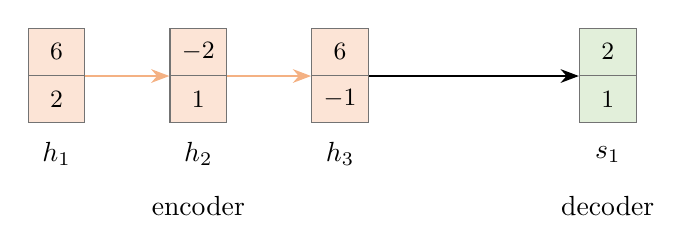
\begin{tikzpicture}[>=Stealth,
            cell/.style={draw=black!55, minimum width=0.72cm, minimum height=0.6cm,
                         inner sep=0pt, font=\small},
            enc/.style={cell, fill=EncFill},
            dec/.style={cell, fill=DecFill}]

            % estados do encoder
            \node[enc] (h1a) at (0, 0.6) {$6$};
            \node[enc] (h1b) at (0, 0)   {$2$};
            \node at (0, -0.7) {$h_1$};

            \node[enc] (h2a) at (1.8, 0.6) {$-2$};
            \node[enc] (h2b) at (1.8, 0)   {$1$};
            \node at (1.8, -0.7) {$h_2$};

            \node[enc] (h3a) at (3.6, 0.6) {$6$};
            \node[enc] (h3b) at (3.6, 0)   {$-1$};
            \node at (3.6, -0.7) {$h_3$};

            % estado do decoder
            \node[dec] (s1a) at (7.0, 0.6) {$2$};
            \node[dec] (s1b) at (7.0, 0)   {$1$};
            \node at (7.0, -0.7) {$s_1$};

            % fluxo recorrente do encoder e ligação com o decoder
            \draw[->, EncArrow, thick] (h1a.south east) -- (h2a.south west);
            \draw[->, EncArrow, thick] (h2a.south east) -- (h3a.south west);
            \draw[->, black, thick]    (h3a.south east) -- (s1a.south west);

            \node at (1.8, -1.35) {encoder};
            \node at (7.0, -1.35) {decoder};
        \end{tikzpicture}
        \caption{Diagrama contemplando os estados ocultos $h_i$ de um \textit{encoder} baseado em RNNs e o estado oculto de um \textit{decoder} $s_1$. A representação dos tokens e dos \textit{embeddings} dos \textit{tokens} foram removidas da figura para simplificar o diagrama.}
        \label{fig:rnn-attention}
    \end{figure}

    \item (Prince, 2024) Considerando que um mecanismo de \textit{self-attention} processa $N$ entradas de tamanho $D$ para produzir $N$ saídas de tamanho $D$.
    Quantos parâmetros treináveis são usados para computar \textit{querys}, \textit{keys} e \textit{values}?
    Caso seja utilizada uma camada linear densa ao invés do mecanismo de atenção, o número de parâmetros treináveis seria maior ou menor?

    \item Qual é o limite teórico do tamanho de sequências que podemos processar com o mecanismo de \textit{self-attention}?

    \item É comum no treinamento e na inferência de \textit{transformers} limitarmos o tamanho das sequências tanto na entrada quanto na saída.
    Qual o motivo disso?

    \item Por que a camada de \textit{self-attention} no \textit{encoder} do \textit{transformer} original não possui máscaras e no \textit{decoder} possui máscaras?

    \item Qual a diferença entre \textit{cross-attention} e \textit{self-attention}?

    \item Qual a vantagem de utilizarmos \textit{multi-head self-attention} em comparação a \textit{self-attention}?

\end{enumerate}

% ============================================================
\section*{Parte 2: Questões Objetivas}
% ============================================================

\paragraph{Instruções:} Cada questão possui exatamente uma alternativa correta.

\begin{enumerate}[I)]
\setcounter{enumi}{8}

% ------------------------------------------------------------------
% Q9 — Fácil (variância do produto escalar e fator de escala)
% ------------------------------------------------------------------
\item Considere dois vetores $S, H \in \mathbb{R}^d$ com componentes
      $s_i, h_i \sim \mathcal{N}(0, 1)$ i.i.d. Para $d = 64$, qual o valor da
      variância de $S \cdot H$ e por qual fator devemos dividir o produto
      escalar para que a variância dos scores resultantes seja igual a~1?

\begin{enumerate}[a)]
    \item $\mathrm{var}[S \cdot H] = 1$, dividir por $1$.
    \item $\mathrm{var}[S \cdot H] = 8$, dividir por $\sqrt{8}$.
    \item $\mathrm{var}[S \cdot H] = 64$, dividir por $\sqrt{64} = 8$.
    \item $\mathrm{var}[S \cdot H] = 64^2$, dividir por $64$.
\end{enumerate}
% R: c

% ------------------------------------------------------------------
% Q10 — Fácil/Médio (variantes de score: dot, bilinear, MLP)
% ------------------------------------------------------------------
\item As três variantes de \textit{score} apresentadas para atenção são
      \textbf{dot-product} ($h^\top s$), \textbf{bilinear} ($h^\top W s$)
      e \textbf{MLP aditiva} ($w_2^\top \tanh(W_1 [h; s])$). Qual afirmação
      compara corretamente as três em termos de parâmetros e custo?

\begin{enumerate}[a)]
    \item A dot-product tem um parâmetro escalar aprendido, a bilinear adiciona
          uma matriz $W$, e a MLP aditiva tem dois conjuntos de pesos.
    \item A dot-product não tem parâmetros aprendidos, a bilinear adiciona uma
          matriz $W$, e a MLP aditiva é a mais expressiva e cara das três.
    \item A dot-product e a bilinear não têm parâmetros aprendidos, e apenas a
          MLP aditiva tem pesos treináveis no score.
    \item As três variantes têm o mesmo número de parâmetros e diferem somente
          no custo computacional do passo \textit{forward}.
\end{enumerate}
% R: b

% ------------------------------------------------------------------
% Q11 — Médio (cálculo de projeção de query)
% ------------------------------------------------------------------
\item Considere o token $x = [1,\;2,\;3]$ e a matriz de projeção
      \[
        W_q = \begin{bmatrix} 2 & 1 \\ 0 & 1 \\ 1 & 0 \end{bmatrix}.
      \]
      Com bias zero, qual o valor de $q = x \, W_q$?

\begin{enumerate}[a)]
    \item $[3,\;2]$
    \item $[5,\;3]$
    \item $[3,\;5]$
    \item $[5,\;5]$
\end{enumerate}
% R: b

% ------------------------------------------------------------------
% Q12 — Médio (saída da atenção como soma ponderada de values)
% ------------------------------------------------------------------
\item Considere os pesos da atenção (já normalizados pela softmax) e a matriz
      de \textit{values} para um \textit{query} fixo:
      \[
        a = [\,0.7,\; 0.2,\; 0.1\,], \qquad
        V = \begin{bmatrix} 10 & 0 \\ 0 & 10 \\ 5 & 5 \end{bmatrix}.
      \]
      Qual é o vetor de contexto $c = \sum_{i=1}^{3} a_i\, V_i$?

\begin{enumerate}[a)]
    \item $[\,15,\;15\,]$
    \item $[\,5.0,\;5.0\,]$
    \item $[\,7.5,\;2.5\,]$
    \item $[\,7.0,\;0.0\,]$
\end{enumerate}
% R: c

% ------------------------------------------------------------------
% Q13 — Médio (por que self-attention "crua" não funciona)
% ------------------------------------------------------------------
\item Considere a versão ``crua'' de \textit{self-attention}, em que aplicamos
      diretamente
      \[
        \mathrm{score}(x_t, x_k) = \frac{x_t^\top x_k}{\sqrt{d}}, \qquad
        c^{(t)} = \sum_{k=1}^{m} a_k^{(t)}\, x_k,
      \]
      sem nenhuma projeção linear sobre os tokens. Qual é o problema dessa
      formulação?

\begin{enumerate}[a)]
    \item O cálculo é determinístico nas entradas e não tem parâmetros
          treináveis no bloco de atenção, então o \textit{backpropagation}
          não tem o que ajustar.
    \item O score $x_t^\top x_k$ é sempre não negativo, fazendo com que a
          softmax sature em pesos próximos a $1/m$.
    \item A normalização por $\sqrt{d}$ deixa de funcionar quando $x_t$ e
          $x_k$ não têm a mesma média componente a componente.
    \item A operação se torna equivalente a uma única camada densa sem
          ativação, removendo a expressividade não linear da atenção.
\end{enumerate}
% R: a

% ------------------------------------------------------------------
% Q14 — Fácil (invariância à permutação sem positional encoding)
% ------------------------------------------------------------------
\item Considere as duas frases a seguir, formadas pelos mesmos \textit{tokens}
      em ordem diferente:
\begin{center}
$S_1$: \texttt{"lucas comeu pastel no jantar"} \\
$S_2$: \texttt{"jantar comeu pastel no lucas"}
\end{center}
      Suponha que ambas sejam processadas por uma camada de \textit{self-attention}
      pura, sem \textit{positional encoding} e sem máscara. O que acontece?

\begin{enumerate}[a)]
    \item As saídas são diferentes, pois o índice $i$ de cada token influencia
          o cálculo das chaves $k_i$.
    \item Para cada token, a saída produzida é a mesma em $S_1$ e em $S_2$
          (apenas em ordem permutada), pois o cálculo independe da posição.
    \item A camada falha por incompatibilidade de dimensões e exige preenchimento
          com \texttt{<PAD>} para alinhar as duas frases.
    \item A softmax dos scores compensa automaticamente a permutação,
          recuperando a ordem original dos \textit{tokens}.
\end{enumerate}
% R: b

% ------------------------------------------------------------------
% Q15 — Médio (multi-head: total de scores de atenção por camada)
% ------------------------------------------------------------------
\item Em uma camada de \textit{multi-head attention} com $H = 8$ cabeças,
      cada cabeça mantém sua própria matriz de scores pré-softmax
      $A^{(h)} = Q^{(h)} (K^{(h)})^\top / \sqrt{d_k}$. Para uma sequência
      de $N = 16$ tokens, quantas entradas escalares (somando todas as cabeças)
      essas matrizes contêm em uma única camada?

\begin{enumerate}[a)]
    \item $16 \cdot 8 = 128$
    \item $16^2 = 256$
    \item $8^2 \cdot 16 = 1\,024$
    \item $16^2 \cdot 8 = 2\,048$
\end{enumerate}
% R: d

% ------------------------------------------------------------------
% Q16 — Médio (LayerNorm vs BatchNorm com sequências de comprimento variável)
% ------------------------------------------------------------------
\item Um pesquisador treina um \textit{transformer} em mini-batches que
      contêm sequências de comprimentos muito variados (de $5$ a $500$
      \textit{tokens}). Por que substituir \textit{LayerNorm} por
      \textit{BatchNorm} levaria a estimativas instáveis de média e variância?

\begin{enumerate}[a)]
    \item BatchNorm computa estatísticas por linha do tensor, então a soma das
          linhas em \textit{batches} grandes diverge para sequências longas.
    \item BatchNorm computa estatísticas por coluna (\textit{feature}) sobre
          o \textit{batch}; com sequências de comprimentos diferentes, o
          número de \textit{tokens} contribuindo em cada posição varia,
          distorcendo as estatísticas.
    \item BatchNorm usa parâmetros aprendidos diferentes de LayerNorm,
          o que requer reinicializar o otimizador a cada novo \textit{batch}.
    \item BatchNorm depende de uma janela deslizante temporal que não está
          disponível em \textit{transformers} sem recorrência.
\end{enumerate}
% R: b

% ------------------------------------------------------------------
% Q17 — Médio (máscara causal e softmax)
% ------------------------------------------------------------------
\item No \textit{decoder}, aplicamos uma máscara causal somando uma matriz
      $M$ aos scores antes da \textit{softmax}. Para a posição $t = 2$
      (que pode atender apenas às posições $1$ e $2$), considere os scores
      \[
        \mathrm{scores}_2 = [\,1.5,\; 0.5,\; 2.0,\; 1.0\,], \qquad
        M_2 = [\,0,\; 0,\; -\infty,\; -\infty\,].
      \]
      Quais são os pesos da atenção $a^{(2)}$ resultantes (após \textit{softmax})?

\begin{enumerate}[a)]
    \item $[\,0.55,\; 0.10,\; 0.25,\; 0.10\,]$
    \item $[\,0.73,\; 0.27,\; 0,\; 0\,]$
    \item $[\,0.25,\; 0.25,\; 0.25,\; 0.25\,]$
    \item $[\,1.5,\; 0.5,\; 0,\; 0\,]$
\end{enumerate}
% R: b

% ------------------------------------------------------------------
% Q18 — Médio (cross-attention: origem de Q, K e V)
% ------------------------------------------------------------------
\item No bloco de \textit{cross-attention} do \textit{decoder} de uma
      arquitetura \textit{encoder-decoder} (por exemplo, em uma tarefa de
      tradução), de onde provêm $Q$, $K$ e $V$?

\begin{enumerate}[a)]
    \item $Q$, $K$ e $V$ vêm todos do \textit{encoder}; o \textit{decoder}
          fornece apenas o sinal de \textit{masking} causal.
    \item $Q$, $K$ e $V$ vêm todos do \textit{decoder}; o \textit{encoder}
          fornece apenas a sequência inicial de \textit{embeddings}.
    \item $Q$ vem do \textit{decoder} e $K, V$ vêm do \textit{encoder};
          a \textit{query} consulta os estados da sequência de origem.
    \item $Q$ vem do \textit{encoder} e $K, V$ vêm do \textit{decoder};
          o sinal flui no sentido oposto ao do \textit{self-attention}
          do \textit{encoder}.
\end{enumerate}
% R: c

% ------------------------------------------------------------------
% Q19 — \emoji{skull-and-crossbones} Difícil (parâmetros do bloco FFN)
% ------------------------------------------------------------------
\item \emoji{skull-and-crossbones} A FFN do \textit{transformer} original é
      definida como
      \[
        \mathrm{FFN}(x) = \mathrm{ReLU}(x W_1 + b_1)\,W_2 + b_2,
      \]
      com $W_1 \in \mathbb{R}^{d \times d_{ff}}$,
      $W_2 \in \mathbb{R}^{d_{ff} \times d}$,
      $b_1 \in \mathbb{R}^{d_{ff}}$ e $b_2 \in \mathbb{R}^{d}$.
      Para $d = 512$ e $d_{ff} = 2\,048$, quantos parâmetros treináveis
      (incluindo \textit{biases}) existem nesse bloco em uma única camada?

\begin{enumerate}[a)]
    \item $2\,097\,152$
    \item $1\,313\,280$
    \item $2\,099\,712$
    \item $4\,194\,304$
\end{enumerate}
% R: c

% ------------------------------------------------------------------
% Q20 — \emoji{skull-and-crossbones} Difícil (custos assintóticos de self-attention)
% ------------------------------------------------------------------
\item \emoji{skull-and-crossbones} Em uma camada de \textit{self-attention}
      processando uma sequência de $N$ tokens com dimensão $d$, ignorando
      \textit{biases}, quais são os custos assintóticos respectivos para:
      (i) a quantidade de parâmetros das matrizes $W_Q, W_K, W_V, W_O$,
      e (ii) o número de operações multiplicar-acumular (FLOPs) para
      computar a matriz de scores $Q K^\top$?

\begin{enumerate}[a)]
    \item (i) $\Theta(d^2)$,\quad (ii) $\Theta(N\, d)$
    \item (i) $\Theta(d^2)$,\quad (ii) $\Theta(N^2\, d)$
    \item (i) $\Theta(N\, d)$,\quad (ii) $\Theta(N^2\, d)$
    \item (i) $\Theta(N^2)$,\quad (ii) $\Theta(N^2\, d^2)$
\end{enumerate}
% R: b

\end{enumerate}

% ============================================================
\newpage
\section*{Gabarito}
% ============================================================
\color{blue}

\subsection*{Parte 1: Questões Discursivas}

\begin{enumerate}[I)]

    \item Ao usar o mecanismo de atenção em uma arquitetura \textit{encoder-decoder} estamos evitando (ou pelo menos minimizando) um gargalo de comunicação entre o \textit{encoder} e o \textit{decoder}. Isso ocorre pois sem a atenção, o \textit{decoder} consegue ter acesso apenas a um estado oculto do \textit{encoder} que deve ser capaz de representar toda a sequência armazenada.

    \item
$
\begin{bmatrix}
6 \\
1.86
\end{bmatrix}
$

\item Cada uma das três componentes da atenção, \textit{query}, \textit{key} e \textit{values} demanda  $D\times D$ parâmetros treináveis mais $D$ bias, sendo o total $3D^2+3D$ para computar todo mecanismo de self-attention. Para fins de comparação, uma camada densa totalmente conectada demandaria $(DN)^2 + DN$ parâmetros treináveis.
Dessa forma percebemos que o número de parâmetros treináveis é menor com o mecanismo de \textit{self-attention}.

\item Não há limite teórico para o tamanho da sequência no processamento por \textit{self-attention}.
Contudo sabemos que existe um custo computacional quadrático em relação ao tamanho da sequência, isso acaba criando limites práticos para o tamanho de sequências que conseguimos processar.
(Podemos ser preciosistas ao responder essa questão e apontar que apesar de conseguir computar a atenção em uma sequência de tamanho arbitrariamente grande, o limite efetivo que conseguimos processar tem relação com o tamanho dos vetores de \textit{query} e \textit{keys}, pois queremos ser capazes de diferenciar a similaridade entre todos os vetores processados).

\item Existem vários motivos para limitarmos o tamanho da sequência tanto em treino quanto em inferência sendo que praticamente todos remetem a questões de eficiência.
Por exemplo, temos que garantir que exista vram suficiente para o treinamento e uma forma de fazer isso é limitando o tamanho das sequências; outra questão importante é garantirmos que o modelo consegue interpretar adequadamente os \textit{positional embeddings}, embora em teoria o modelo deva ser capaz de generalizar para sequências maiores na prática isso pode não ocorrer; Durante o treinamento queremos ser capazes de colocar todas as sentenças de um \textit{batch} em um único tensor, para permitir esse processo é comum completarmos sequências mais curtas com \texttt{<PAD>} para facilitar esse processo limitamos o tamanho das sequências e também implementamos um processo de \textit{bucketing}.

\item Durante o \textit{treino} com \textit{teacher forcing}, o \textit{decoder} recebe toda a sequência alvo de uma só vez, em paralelo. A máscara causal impede que a posição $t$ veja as posições futuras $t+1, t+2, \ldots$ ao computar a atenção, garantindo que cada predição use apenas o contexto que estará disponível em inferência (autoregressiva). Sem a máscara, o modelo simplesmente copiaria o próximo \textit{token} da sequência alvo (trapaceando) e não aprenderia a prever. O \textit{encoder}, ao contrário, processa a frase de entrada de uma só vez e toda ela está disponível ao mesmo tempo, então não há razão para mascarar.

\item Em \textit{Cross-attention} as querys e \textit{keys} vem de sequências diferentes enquanto que em \textit{self-attention} as \textit{querys} e \textit{keys} vem da mesma sequência.

\item A principal vantagem é representacional: cada cabeça aprende a atender a um \textbf{tipo de relação diferente} entre os \textit{tokens} da sequência, por exemplo, relações sintáticas (sujeito-verbo, modificador-substantivo), semânticas (referente de um pronome), posicionais (próximo \textit{token}) ou de longo alcance. Trabalhos como \textit{Voita et al.\ (2019)} \textit{Analyzing Multi-Head Self-Attention} mostram empiricamente que cabeças individuais especializam-se em diferentes funções linguísticas. Como benefício secundário, o cômputo das múltiplas cabeças é trivialmente paralelizável (operação \textit{batched} em GPU), mas esse não é o motivo principal, uma única cabeça de mesma dimensão total seria igualmente paralelizável.

\end{enumerate}

\subsection*{Parte 2: Questões Objetivas}

% --- Solução Q9 ---
\subsubsection*{IX — Resposta: (c)}
Como $s_i, h_i \sim \mathcal{N}(0, 1)$ são independentes,
$\mathbb{E}[s_i] = \mathbb{E}[h_i] = 0$ e $\mathrm{var}(s_i) = \mathrm{var}(h_i) = 1$.
Assim,
\[
  \mathrm{var}[S \cdot H]
    = \sum_{i=1}^{d} \mathrm{var}(s_i\, h_i)
    = \sum_{i=1}^{d} \mathbb{E}[s_i^2]\,\mathbb{E}[h_i^2]
    = \sum_{i=1}^{d} 1 = d.
\]
Para $d = 64$, $\mathrm{var}[S \cdot H] = 64$. Para reescalar o desvio
padrão a $1$, dividimos por $\sqrt{64} = 8 = \sqrt{d}$, justamente o fator de
escala usado pela \textit{scaled dot product attention}.
A opção~(a) ignora que somamos $d$ termos com variância~1. A opção~(b) confunde
$d$ com $\sqrt{d}$. A opção~(d) eleva o resultado ao quadrado.
% ---

% --- Solução Q10 ---
\subsubsection*{X — Resposta: (b)}
A variante \textbf{dot-product} ($h^\top s$) não introduz parâmetros
aprendidos: o score depende apenas dos vetores que entram no cálculo. A
\textbf{bilinear} ($h^\top W s$) adiciona uma matriz $W$ aprendida que
atua como um produto interno paramétrico. A \textbf{MLP aditiva}
($w_2^\top \tanh(W_1 [h; s])$) tem dois conjuntos de pesos $W_1, w_2$
e ainda computa um $\tanh$ por par $(h, s)$, sendo a mais cara das três.
A opção~(a) atribui erroneamente um parâmetro à dot-product. A opção~(c)
esquece que a bilinear tem $W$. A opção~(d) ignora as diferenças óbvias
de número de parâmetros.
% ---

% --- Solução Q11 ---
\subsubsection*{XI — Resposta: (b)}
A multiplicação $q = x\, W_q$ produz um vetor de duas componentes:
\[
  q_0 = 1\cdot 2 + 2\cdot 0 + 3\cdot 1 = 5, \qquad
  q_1 = 1\cdot 1 + 2\cdot 1 + 3\cdot 0 = 3.
\]
Logo $q = [5,\;3]$.
A opção~(a) corresponde a somar as colunas de $W_q$ ignorando $x$:
$[2+0+1,\,1+1+0] = [3,\,2]$. A opção~(c) inverte os componentes. A
opção~(d) usa a primeira coluna de $W_q$ para ambas as posições da saída
($1\cdot 2 + 2\cdot 0 + 3\cdot 1 = 5$ aplicado duas vezes).
% ---

% --- Solução Q12 ---
\subsubsection*{XII — Resposta: (c)}
O contexto é a soma das linhas de $V$ ponderada por $a$:
\[
  c = 0.7 \cdot [10,\,0] + 0.2 \cdot [0,\,10] + 0.1 \cdot [5,\,5]
    = [7,\,0] + [0,\,2] + [0.5,\,0.5]
    = [7.5,\;2.5].
\]
A opção~(a) soma as linhas de $V$ sem usar os pesos $a$. A opção~(b)
distribui peso uniforme $1/3$ entre as linhas. A opção~(d) aplica apenas
o peso $a_1 = 0.7$ à primeira linha de $V$ e ignora os demais
\textit{values}.
% ---

% --- Solução Q13 ---
\subsubsection*{XIII — Resposta: (a)}
Sem as projeções $W_q$, $W_k$, $W_v$, o cálculo de scores e do contexto
depende apenas dos próprios \textit{embeddings} de entrada. Não há
parâmetros do bloco de atenção que possam ser ajustados durante o
treinamento, logo o \textit{backpropagation} não tem o que aprender ali.
A solução é introduzir as três projeções lineares $q_t = x_t W_q$,
$k_t = x_t W_k$, $v_t = x_t W_v$, criando os parâmetros que serão
otimizados.
A opção~(b) é falsa: $x_t^\top x_k$ pode ser negativo, dependendo dos
\textit{embeddings}. A opção~(c) inventa um problema com a média que
não existe. A opção~(d) confunde ausência de parâmetros com ausência de
não-linearidade: a softmax permanece não linear mesmo no caso ``cru''.
% ---

% --- Solução Q14 ---
\subsubsection*{XIV — Resposta: (b)}
Sem \textit{positional encoding}, os vetores $q_t$, $k_t$ e $v_t$
dependem apenas do \textit{token} (do conteúdo de $x_t$), não da posição
$t$. As duas frases $S_1$ e $S_2$ contêm exatamente o mesmo conjunto de
\textit{tokens}, apenas em ordem distinta: portanto o conjunto de
$(q_i, k_i, v_i)$ é o mesmo. Para o \textit{token} ``comeu'' (que ocupa
a mesma posição em $S_1$ e $S_2$), os scores e o contexto resultante são
idênticos. Para os demais \textit{tokens} permutados, a saída é a mesma
em ambas as frases, apenas reordenada. Em outras palavras, a camada é
\emph{permutation equivariant}, motivo pelo qual o \textit{positional
encoding} é necessário.
A opção~(a) atribui a $k_i$ uma dependência do índice que não existe sem
PE. A opção~(c) inventa um erro de dimensão. A opção~(d) atribui à
softmax uma capacidade de recuperar ordem que ela não possui.
% ---

% --- Solução Q15 ---
\subsubsection*{XV — Resposta: (d)}
Cada cabeça de \textit{self-attention} produz uma matriz de scores
$N \times N$ com $N^2 = 256$ entradas. Com $H = 8$ cabeças trabalhando em
paralelo, há $256 \cdot 8 = 2\,048$ scores escalares por camada.
A opção~(a) é apenas $N \cdot H$ (ignora a dependência quadrática em $N$).
A opção~(b) considera somente uma cabeça. A opção~(c) inverte os papéis
de $H$ e $N$ ($H^2 \cdot N$).
% ---

% --- Solução Q16 ---
\subsubsection*{XVI — Resposta: (b)}
\textit{BatchNorm} computa média e variância \emph{por feature}, agregando
sobre o eixo do \textit{batch} e (em sequências) sobre o eixo temporal.
Com sequências de comprimentos muito distintos, o número de \textit{tokens}
que contribuem para cada posição varia: posições próximas ao início
acumulam centenas de amostras, enquanto posições próximas ao fim recebem
apenas algumas. As estatísticas resultantes ficam ruidosas e dependentes
da composição do \textit{batch}. \textit{LayerNorm}, por outro lado,
normaliza \emph{por token} (linha), independendo do tamanho do
\textit{batch} ou do comprimento das sequências.
A opção~(a) inverte o eixo de normalização do BatchNorm. A opção~(c)
inventa um requisito de reinicialização do otimizador que não existe.
A opção~(d) atribui ao BatchNorm uma janela deslizante que não faz parte
da sua definição.
% ---

% --- Solução Q17 ---
\subsubsection*{XVII — Resposta: (b)}
Após somar a máscara, os scores efetivos passam a ser
$[\,1.5,\; 0.5,\; -\infty,\; -\infty\,]$. Aplicando $\exp$:
\[
  e^{1.5} \approx 4.482, \quad
  e^{0.5} \approx 1.649, \quad
  e^{-\infty} = 0.
\]
A soma é $4.482 + 1.649 = 6.131$, então
\[
  a^{(2)} = \left[\frac{4.482}{6.131},\; \frac{1.649}{6.131},\; 0,\; 0\right]
         \approx [\,0.73,\; 0.27,\; 0,\; 0\,].
\]
A opção~(a) ignora a máscara, aplicando \textit{softmax} aos quatro
scores originais. A opção~(c) atribui peso uniforme. A opção~(d)
apenas anula as duas últimas entradas e mantém os scores brutos no lugar
das probabilidades.
% ---

% --- Solução Q18 ---
\subsubsection*{XVIII — Resposta: (c)}
Em \textit{cross-attention} (também chamado \textit{encoder-decoder
attention}), a \textit{query} é construída a partir do estado atual do
\textit{decoder} (``o que estou gerando agora''), enquanto \textit{keys}
e \textit{values} vêm da saída do \textit{encoder} (``o que está na
sequência de origem''). Em uma tarefa de tradução, ao gerar a palavra
``cat'' o \textit{decoder} emite uma \textit{query} que consulta as
\textit{keys} do \textit{encoder} e atende aos \textit{values}
correspondentes ao \textit{token} ``gato'' na frase original.
A opção~(a) inverte o papel do \textit{decoder}. A opção~(b) coincidiria
com \textit{self-attention} do próprio \textit{decoder}, não com
\textit{cross-attention}. A opção~(d) inverte os papéis de $Q$ e $K, V$.
% ---

% --- Solução Q19 ---
\subsubsection*{XIX — Resposta: (c)}
Contagem direta dos parâmetros:
\[
  |W_1| = d \cdot d_{ff} = 512 \cdot 2\,048 = 1\,048\,576,
\]
\[
  |W_2| = d_{ff} \cdot d = 2\,048 \cdot 512 = 1\,048\,576,
\]
\[
  |b_1| = d_{ff} = 2\,048, \qquad |b_2| = d = 512.
\]
Total:
\[
  1\,048\,576 + 1\,048\,576 + 2\,048 + 512 = 2\,099\,712.
\]
A opção~(a) ignora os \textit{biases}: $2\cdot 512\cdot 2\,048 = 2\,097\,152$.
A opção~(b) usa $W_2 \in \mathbb{R}^{d\times d}$ por engano:
$1\,048\,576 + 262\,144 + 2\,048 + 512 = 1\,313\,280$.
A opção~(d) duplica indevidamente o número de matrizes:
$4\cdot 512\cdot 2\,048 = 4\,194\,304$.
% ---

% --- Solução Q20 ---
\subsubsection*{XX — Resposta: (b)}
\textbf{(i)~Parâmetros das projeções.} Cada uma das matrizes $W_Q$, $W_K$,
$W_V$ e $W_O$ tem formato $d \times d$, contribuindo $d^2$ parâmetros, em
um total de $4d^2 = \Theta(d^2)$. Note que esse total \emph{não depende}
de $N$, propriedade central da atenção em comparação a uma camada densa
sobre toda a sequência.

\textbf{(ii)~FLOPs para $Q K^\top$.} Com $Q \in \mathbb{R}^{N\times d}$ e
$K^\top \in \mathbb{R}^{d\times N}$, o resultado é uma matriz $N\times N$ na
qual cada entrada $(i, j)$ é o produto interno entre uma linha de $Q$ e
uma coluna de $K^\top$, custando $d$ multiplicações-adições. Total:
$N^2 \cdot d = \Theta(N^2\, d)$.

A opção~(a) subestima o custo de $QK^\top$ ao ignorar a dependência
quadrática em $N$. A opção~(c) faz os parâmetros escalarem com $N$,
contradizendo a propriedade de invariância em comprimento da atenção.
A opção~(d) infla parâmetros e FLOPs por confundir os dois regimes.
% ---

\end{document}
